\chapter{Двухэтапный конвейер обеспечения безопасности мультимодальных LLM}\label{ch:safety}

Промышленное развёртывание больших языковых и мультимодальных моделей требует надёжных механизмов обеспечения безопасности, устойчивых к разнообразным атакам, систематизированным в обзоре литературы (Разделы~\ref{sec:ai_safety} и~\ref{sec:vulnerabilities}).
В настоящей главе представлен двухэтапный конвейер обеспечения безопасности, объединяющий потоковый классификатор обменов на основе предобученной MoE-модели GigaChat3.1-10B-A1.8B~\cite{gigachat3_10b} и безопасную языковую модель, дообученную методом обучения с подкреплением с наградой за безопасность.
Конвейер интегрирует поисковый стек, развитый в Главах~\ref{ch:gigaembeddings}--\ref{ch:rag}, в виде инструмента безопасного поиска по курируемому индексу, обеспечивая защищённой модели актуальный и достоверный взгляд на предметную область.
Изложение опирается на серию работ по конституционному ИИ и обучению безопасных ассистентов~\cite{bai2022cai,bai2022hhrlhf,sharma2025cc,cunningham2026ccpp} и на подход к проектированию награды за безопасность, предложенный в Qwen3Guard~\cite{2510.14276}.

%% =================================================================
\section{Мотивация и принципы проектирования}\label{sec:sp_motivation}
%% =================================================================

Архитектура конвейера руководствуется тремя основными принципами.

\textbf{Классификация на уровне обмена.} В отличие от раздельной модерации входного запроса и выходного ответа, классификатор оценивает обмен (exchange) целиком --- пользовательский запрос совместно с порождаемым префиксом ответа защищаемой модели.
Контекстная оценка ответа в связке с запросом устойчива к атакам, распределяющим вредоносное содержание между модальностями или фрагментами (reconstruction attacks), и к атакам с обфускацией вывода~\cite{cunningham2026ccpp}.

\textbf{Независимость защитного слоя.} Классификатор реализован как самостоятельная модель, не использующая внутренние активации защищаемой модели.
Это устраняет необходимость перекалибровки защитного слоя при каждом обновлении, квантовании или дообучении защищаемой модели и позволяет развивать обе компоненты независимо.

\textbf{Эшелонированная защита.} Конвейер реализует многослойную оборону: быстрый потоковый классификатор фильтрует основной поток трафика, а безопасная модель формирует неуклончивые ответы на заблокированные запросы.
Подобная организация согласуется с принципом <<швейцарского сыра>>, лежащим в основе конституционных классификаторов~\cite{sharma2025cc}.

%% =================================================================
\section{Общая архитектура конвейера}\label{sec:sp_architecture}
%% =================================================================

Конвейер состоит из двух этапов (Рисунок~\ref{fig:safety_pipeline}).
На первом этапе потоковый классификатор оценивает обмен в реальном времени, относя его к одной из трёх зон: пропуск (pass), мониторинг (monitor) или блокировка (block).
На втором этапе запросы, отнесённые к зоне блокировки, обрабатываются безопасной моделью, формирующей корректный отказ или безопасный ответ с опорой на инструмент безопасного поиска.

\begin{figure}[htbp]
    \centering
    \resizebox{0.97\textwidth}{!}{
        \begin{tikzpicture}[
    font=\sffamily,
    node distance=1.1cm and 1.8cm,
    box/.style={
        draw,
        rounded corners,
        minimum width=3.2cm,
        minimum height=1.1cm,
        align=center,
        thick
    },
    big/.style={
        draw,
        rounded corners,
        minimum width=4.0cm,
        minimum height=1.4cm,
        align=center,
        very thick
    },
    small/.style={
        draw,
        rounded corners,
        minimum width=2.7cm,
        minimum height=1.0cm,
        align=center,
        thick
    },
    arr/.style={-{Stealth[length=3mm]}, thick}
]
    %% Вход
    \node[box] (req) {Запрос +\\ответ модели};
    %% Этап 1
    \node[big, right=of req] (clf) {Этап~1:\\потоковый\\MoE-классификатор\\(GigaChat-10B)};
    %% Три зоны решения
    \node[small, right=2.2cm of clf] (pass) {pass\\(стриминг)};
    \node[small, above=of pass] (monitor) {monitor\\(аудит)};
    \node[small, below=of pass] (block) {block};
    %% Этап 2
    \node[big, below=1.1cm of block] (safe) {Этап~2:\\безопасная модель\\(RLHF, safe-search)};
    %% Очередь аудита
    \node[small, above=1.0cm of monitor] (audit) {Офлайн-аудит\\и дообучение};

    %% Стрелки
    \draw[arr] (req) -- (clf);
    \draw[arr] (clf) -- node[above, font=\small] {$\bar p < \tau_{m}$} (pass);
    \draw[arr] (clf) -- node[left, font=\small, pos=0.6] {$\tau_{m}\le\bar p\le\tau_{b}$} (monitor);
    \draw[arr] (clf) -- node[left, font=\small, pos=0.6] {$\bar p > \tau_{b}$} (block);
    \draw[arr] (monitor) -- (audit);
    \draw[arr] (block) -- (safe);
    \draw[arr] (audit) to[bend right=35] (clf);
\end{tikzpicture}

    }
    \caption{Двухэтапный конвейер обеспечения безопасности: потоковый MoE-классификатор с тремя зонами решения и безопасная модель, дообученная с подкреплением.}
    \label{fig:safety_pipeline}
\end{figure}

При отказе классификатора применяется одна из двух политик отказоустойчивости: <<отказ в безопасную сторону>> (fail-closed), маршрутизирующий весь трафик на безопасную модель, либо <<отказ с правилами>> (fail-open), применяющий упрощённую фильтрацию на основе правил.
Запросы из зоны мониторинга направляются в офлайн-очередь для последующего экспертного анализа и обогащения обучающей выборки.

%% =================================================================
\section{Этап 1: классификатор на основе GigaChat-10B MoE}\label{sec:sp_stage1}
%% =================================================================

\subsection{Генеративная адаптация классификатора}\label{subsec:sp_generative}

В качестве основы классификатора используется базовая предобученная (pretrain) модель GigaChat3.1-10B-A1.8B~\cite{gigachat3_10b} --- отдельная языковая модель семейства GigaChat с архитектурой Mixture of Experts (Раздел~\ref{subsec:gc_moe}).
Модель построена на архитектуре, близкой к DeepSeek~V3~\cite{deepseek2025v3}, сочетающей механизм латентного внимания (Multi-Head Latent Attention, MLA) с разреженной смесью экспертов.
Из приблизительно 10 миллиардов общих параметров при разреженной маршрутизации активируется лишь около 1.8 миллиарда: каждый токен направляется к 4 из 64 маршрутизируемых экспертов наряду с одним общим экспертом (первый слой оставлен плотным), что обеспечивает низкую задержку инференса при высокой ёмкости модели и поддержке длинного контекста (до 256 тысяч токенов).
В отличие от подходов с линейным классификационным зондом по активациям, задача формулируется как предсказание следующего токена.
Шаблон $T(\cdot)$ дополняет обмен служебным маркером, после которого целевым токеном является <<harmful>> либо <<safe>>.
Вероятность вредоносности на позиции $t$ определяется как:
\begin{equation}
\label{eq:sp_pclf}
    p_{\text{clf}}(t) = \mathrm{softmax}\big(\mathrm{LM}_{\text{MoE}}(T(x_{1:t}))\big)_{\text{harmful}},
\end{equation}
где $x_{1:t}$ --- обмен, наблюдаемый до позиции $t$ (запрос и префикс ответа).
Для устойчивости к локальным флуктуациям применяется экспоненциальное скользящее усреднение (exponential moving average, EMA) оценки по токенам:
\begin{equation}
\label{eq:sp_ema}
    \bar{p}_t = \alpha \cdot p_{\text{clf}}(t) + (1 - \alpha) \cdot \bar{p}_{t-1}, \qquad \alpha \in [0.1, 0.3].
\end{equation}
Решение принимается по двум порогам $\tau_{\text{monitor}}$ и $\tau_{\text{block}}$ над сглаженной оценкой $\bar{p}_t$:
\begin{equation}
\label{eq:sp_decision}
    \mathrm{decision}(\bar{p}_t) =
    \begin{cases}
        \text{pass}, & \bar{p}_t < \tau_{\text{monitor}}, \\
        \text{monitor}, & \tau_{\text{monitor}} \le \bar{p}_t \le \tau_{\text{block}}, \\
        \text{block}, & \bar{p}_t > \tau_{\text{block}}.
    \end{cases}
\end{equation}
Пороги калибруются по производственному трафику так, чтобы доля блокировок не превышала $0.05\%$, а доля зоны мониторинга составляла $1$--$3\%$; лишь порог блокировки влияет на пользовательский опыт.

\subsection{Данные и таксономия рисков}\label{subsec:sp_data}

Таксономия рисков охватывает несколько доменов вреда (химические, биологические, радиологические и ядерные угрозы, кибероперации, насилие), причём для каждого вредоносного домена определяется парная безвредная категория.
Намеренная асимметрия --- узкие вредоносные категории и широкие безвредные --- формирует точную границу решения и предотвращает чрезмерную блокировку (over-refusal)~\cite{sharma2025cc}.
Обучающая выборка формируется из нескольких источников: синтетических обменов, порождённых на основе конституции; аугментированных примеров (свыше тридцати типов лингвистических, кодирующих, структурных и ролевых преобразований, включая многопримерные атаки с длинным контекстом~\cite{anil2024manyshot}); успешных атак автоматизированного и ручного состязательного тестирования~\cite{ganguli2022redteam}; а также пула безвредных запросов.

\subsection{Специфика MoE и вычислительная эффективность}\label{subsec:sp_moe}

Потоковая классификация выполняется инкрементально: после однократного префиксного заполнения (prefill) для каждого порождаемого защищаемой моделью токена выполняется один разреженный шаг декодирования с использованием кэша ключей и значений.
Разреженная активация экспертов обеспечивает относительные накладные расходы защитного слоя на уровне единиц процентов от стоимости инференса защищаемой модели.
Сопоставление с конституционными классификаторами~\cite{sharma2025cc,cunningham2026ccpp} показывает, что классификация на уровне обмена обеспечивает существенно меньшее число высокорисковых уязвимостей на одну попытку атаки по сравнению с раздельной модерацией входа и выхода.

В качестве ориентира для оценки качества классификатора используются результаты Qwen3Guard~\cite{2510.14276} (Таблица~\ref{tab:sp_qwen3guard}), демонстрирующие, что компактные модели безопасности достигают качества, превосходящего значительно более крупные базовые линии.

\begin{table}[H]
    \centering
    \caption{Среднее значение F1 на англоязычных бенчмарках безопасности для классификации запросов и ответов. Источник: \cite{2510.14276}.}
    \label{tab:sp_qwen3guard}
    \begin{tabular}{lcc}
        \toprule
        Модель & Запросы (avg F1) & Ответы (avg F1) \\
        \midrule
        Llama Guard 3 (8B)~\cite{2312.06674}   & 79.4 & 70.7 \\
        ShieldGemma (9B)~\cite{2407.21772}      & 70.4 & 62.2 \\
        WildGuard (7B)                          & 85.8 & 79.9 \\
        \midrule
        Qwen3Guard-0.6B                         & 88.1 & 82.0 \\
        Qwen3Guard-4B                           & 89.3 & 83.7 \\
        Qwen3Guard-8B                           & 90.0 & 83.9 \\
        \bottomrule
    \end{tabular}
\end{table}

%% =================================================================
\section{Мультимодальное расширение классификатора}\label{sec:sp_multimodal}
%% =================================================================

Базовая архитектура классификатора оперирует текстовыми обменами, тогда как мультимодальные модели подвержены атакам через визуальный канал (Раздел~\ref{subsec:jailbreak_attacks}): вредоносное содержание может быть закодировано в изображении, типографическом тексте на изображении или в структуре загружаемого файла.
Для покрытия визуального канала классификатор дополняется тремя механизмами.
Во-первых, преобразование изображения в текст (image-to-text) в духе подхода ECSO~\cite{2403.09572} переводит потенциально небезопасное визуальное содержание в текстовое описание, активируя текстовый классификатор обменов.
Во-вторых, оптическое распознавание символов противодействует типографическим атакам, извлекая встроенный в изображение текст для последующей классификации.
В-третьих, скрининг представлений визуального энкодера позволяет выявлять состязательные возмущения изображений до их передачи языковой модели.
Безопасный индекс (Раздел~\ref{sec:sp_safe_search}) при этом покрывает мультимодальные документы, обеспечивая согласованную фильтрацию контента независимо от модальности.

%% =================================================================
\section{Этап 2: безопасная модель (RLHF с наградой за безопасность)}\label{sec:sp_stage2}
%% =================================================================

Второй этап конвейера составляет безопасная языковая модель, формирующая корректные неуклончивые ответы на заблокированные запросы.
Её обучение объединяет тёплый старт методом конституционного ИИ и обучение с подкреплением с наградой за безопасность.

\subsection{Тёплый старт методом конституционного ИИ}\label{subsec:sp_cai}

На этапе обучения с учителем применяется процедура самокритики и переписывания (critique-and-revision) конституционного ИИ~\cite{bai2022cai}: модель, оптимизированная на полезность, порождает ответ на состязательный запрос, затем критикует его в соответствии со случайно выбранным принципом конституции и переписывает, устраняя вредоносность.
Дообучение на финальных переписанных ответах формирует модель, склонную не к уклончивым отказам, а к содержательному объяснению причин отказа.
На этапе обучения с подкреплением метки предпочтений по безопасности порождаются моделью обратной связи (RL from AI Feedback, RLAIF) с использованием мягких меток и ансамблирования по принципам конституции, тогда как метки полезности предоставляются человеком~\cite{bai2022cai,bai2022hhrlhf}.

\subsection{Дизайн награды за безопасность}\label{subsec:sp_reward}

Центральным элементом обучения является конструкция награды.
Следуя подходу Qwen3Guard~\cite{2510.14276}, генеративный классификатор безопасности используется как источник сигнала вознаграждения при оптимизации политики, причём предикат $\mathrm{is\_safe}(\cdot)$ истинен тогда и только тогда, когда классификатор относит содержание к категории <<safe>> (как спорное, так и небезопасное содержание считаются небезопасными).
Простейшая формулировка вознаграждает только безопасность как мышления (thinking) $t$, так и финального ответа $y$ для запроса $x$:
\begin{equation}
\label{eq:sp_reward_guard}
    r(x, t, y) =
    \begin{cases}
        1.0, & \mathrm{is\_safe}(x, t) \wedge \mathrm{is\_safe}(x, y), \\
        0.0, & \text{иначе}.
    \end{cases}
\end{equation}
Награда вида~(\ref{eq:sp_reward_guard}) обеспечивает почти идеальную безопасность, однако приводит к вырожденному поведению --- чрезмерно высокой доле отказов.
Для устранения данного эффекта применяется гибридная награда, совмещающая безопасность с полезностью, оцениваемой отдельной моделью предпочтений $\mathrm{PM}(\cdot)$, и штрафующая необоснованные отказы:
\begin{equation}
\label{eq:sp_reward_hybrid}
    r(x, t, y) =
    \begin{cases}
        \min(-10,\ \mathrm{PM}(x, y)), & \mathrm{is\_unsafe}(x, t) \vee \mathrm{is\_unsafe}(x, y), \\
        \min(-5,\ \mathrm{PM}(x, y)), & \mathrm{is\_refusal}(x, y), \\
        \mathrm{PM}(x, y), & \text{иначе}.
    \end{cases}
\end{equation}
Небезопасное содержание получает сильный штраф (не выше $-10$), необоснованный отказ --- умеренный штраф (не выше $-5$), что подавляет чрезмерную блокировку, тогда как в остальных случаях сохраняется оценка полезности.
Влияние конструкции награды иллюстрирует Таблица~\ref{tab:sp_reward}: награда только за безопасность доводит безопасность до $100\%$ ценой почти полного отказа от ответов, тогда как гибридная награда сохраняет высокую безопасность при низкой доле отказов.

\begin{table}[H]
    \centering
    \caption{Влияние конструкции награды на безопасность и долю отказов модели Qwen3-4B (режим без размышлений). Источник: \cite{2510.14276}.}
    \label{tab:sp_reward}
    \begin{tabular}{lcc}
        \toprule
        Конфигурация & Безопасность (WildGuard) & Доля отказов \\
        \midrule
        Базовая модель               & 64.7  & 12.9 \\
        + награда только безопасность & 100.0 & 96.6 \\
        + гибридная награда           & 98.1  & 5.3  \\
        \bottomrule
    \end{tabular}
\end{table}

\subsection{Алгоритм оптимизации}\label{subsec:sp_rl}

Оптимизация политики выполняется методом проксимальной оптимизации политики (Proximal Policy Optimization, PPO)~\cite{schulman2017ppo} или его групповыми вариантами.
Для предотвращения чрезмерного отклонения политики $\pi$ от референсной модели $\pi_0$ и связанного с ним переоптимизирования награды (reward hacking) к вознаграждению добавляется штраф на расхождение Кульбака--Лейблера~\cite{bai2022hhrlhf}:
\begin{equation}
\label{eq:sp_ppo_kl}
    r_{\text{total}}(x, y) = r(x, t, y) - \lambda_{\text{KL}} \cdot D_{\mathrm{KL}}\big(\pi(\cdot \mid x) \,\|\, \pi_0(\cdot \mid x)\big),
\end{equation}
где $\lambda_{\text{KL}}$ регулирует силу штрафа.
Итеративное онлайн-дообучение, при котором модель предпочтений и политика периодически переобучаются на свежих данных, повышает робастность награды в области высоких оценок, в которую смещается политика по мере обучения~\cite{bai2022hhrlhf}.

%% =================================================================
\section{Инструмент безопасного поиска и безопасный индекс}\label{sec:sp_safe_search}
%% =================================================================

Безопасная модель дополняется инструментом безопасного поиска (safe-search-tool), обеспечивающим доступ к актуальной и проверенной информации (Рисунок~\ref{fig:safe_search_tool}).
Данный инструмент представляет собой точку синтеза поисковой и защитной частей настоящего исследования.

\begin{figure}[htbp]
    \centering
    \resizebox{0.95\textwidth}{!}{
        \begin{tikzpicture}[
    font=\sffamily,
    node distance=1.2cm and 1.9cm,
    box/.style={
        draw,
        rounded corners,
        minimum width=3.0cm,
        minimum height=1.1cm,
        align=center,
        thick
    },
    big/.style={
        draw,
        rounded corners,
        minimum width=3.4cm,
        minimum height=1.4cm,
        align=center,
        very thick
    },
    db/.style={
        draw,
        cylinder,
        shape border rotate=90,
        aspect=0.3,
        minimum width=2.4cm,
        minimum height=1.8cm,
        align=center,
        thick
    },
    arr/.style={-{Stealth[length=3mm]}, thick}
]
    %% Безопасная модель
    \node[big] (safe) {Безопасная\\модель};
    %% Инструмент поиска
    \node[box, right=of safe] (tool) {safe-search-tool\\(двухэтапный поиск)};
    %% Безопасный индекс
    \node[db, right=of tool] (index) {Безопасный\\индекс};
    %% Курирование индекса
    \node[box, above=1.2cm of index] (curate) {Фильтрация\\классификатором\\этапа~1};
    \node[db, above=1.1cm of curate, minimum height=1.4cm] (raw) {Свежие\\данные};
    %% Ответ
    \node[box, below=1.2cm of safe] (answer) {Ответ с\\заземлением};

    %% Стрелки
    \draw[arr] (safe) -- node[above, font=\small] {вызов} (tool);
    \draw[arr] (tool) -- node[above, font=\small] {запрос} (index);
    \draw[arr] (index) to[bend left=20] node[below, font=\small] {top-$n$} (tool);
    \draw[arr] (tool) to[bend left=20] node[below, font=\small] {контекст} (safe);
    \draw[arr] (raw) -- (curate);
    \draw[arr] (curate) -- (index);
    \draw[arr] (safe) -- (answer);
\end{tikzpicture}

    }
    \caption{Инструмент безопасного поиска: безопасная модель обращается к курируемому безопасному индексу через двухэтапный поиск, формируя заземлённый ответ.}
    \label{fig:safe_search_tool}
\end{figure}

\textbf{Построение безопасного индекса.} Безопасный индекс формируется из свежих релевантных документов, проходящих фильтрацию классификатором первого этапа (Раздел~\ref{sec:sp_stage1}): документы, отнесённые к небезопасным, исключаются из индекса.
Тем самым информационное пространство, доступное модели, ограничивается заранее проверенным содержанием, что согласуется с преимуществами RAG в части контролируемости и верифицируемости (Раздел~\ref{sec:rag_motivation}).

\textbf{Доступ через двухэтапный поиск.} Извлечение из безопасного индекса реализуется двухэтапным поисковым стеком (Глава~\ref{ch:rag}): гибридный поиск формирует множество кандидатов, которое уточняется кросс-энкодером (Глава~\ref{ch:reranking}).
Инструмент предоставляется модели в режиме вызова инструментов (tool-calling): модель формирует поисковый запрос, получает заземляющий контекст и порождает ответ с опорой на проверенные источники.

\textbf{Назначение.} Сочетание генерации с извлечением информации и фильтрации по безопасности обеспечивает защищённой модели актуальный взгляд на предметную область без переобучения (Раздел~\ref{sec:rag_motivation}) и без риска извлечения вредоносного или недостоверного контента.
Так поисковый стек, развитый в Главах~\ref{ch:gigaembeddings}--\ref{ch:rag}, непосредственно интегрируется в конвейер обеспечения безопасности больших языковых моделей.

%% =================================================================
\section{Оценка и состязательное тестирование}\label{sec:sp_evaluation}
%% =================================================================

Оценка конвейера проводится в два этапа.
На офлайн-этапе измеряются качество классификатора (доля блокировок и зоны мониторинга, доля высокорисковых уязвимостей), а также безопасность и полезность защищённой модели.
На этапе развёртывания применяются теневое развёртывание (shadow deployment) и поэтапный вывод в продуктив с непрерывным состязательным тестированием.
Программа состязательного тестирования организована по модели вознаграждаемого поиска уязвимостей (bug bounty)~\cite{sharma2025cc,cunningham2026ccpp,ganguli2022redteam}: ответ считается успешно взломанным, если по экспертной рубрике он раскрывает не менее половины детализации незащищённой модели, а высокорисковой уязвимостью --- атака, отвечающая на большинство целевых вредоносных запросов.
\subsection{Эволюция классификатора: от модерации запроса к потоковой оценке ответа}\label{subsec:sp_censor_evolution}

В исходной версии конвейера защитный слой реализовывал модерацию исключительно на уровне запроса (классификатор запросов): решение о блокировке принималось по тексту пользовательского обращения до начала генерации.
Такая схема проста и обладает минимальной задержкой, однако присваивает метку вредоносности самому запросу, тогда как фактический риск определяется порождаемым ответом.
Опираясь на конституционные классификаторы Anthropic~\cite{sharma2025cc,cunningham2026ccpp}, в которых выходной классификатор работает в потоковом режиме над генерируемым ответом, мы перешли от модерации запроса к потоковой оценке ответа --- классификации обмена по мере его порождения (Раздел~\ref{sec:sp_motivation}, принцип классификации на уровне обмена).

Необходимость перехода выявилась при пересмотре методики оценки.
Исходный тестовый набор размечался по запросу, что неявно предполагало совпадение вредоносности запроса и ответа.
На практике это предположение нарушается в обе стороны: защищаемая модель в ряде случаев формирует безопасный ответ на внешне небезопасный запрос (корректный отказ или содержательное объяснение), и наоборот --- внешне безобидный запрос способен спровоцировать небезопасный ответ.
Пересмотренный тестовый набор размечался по фактической безопасности порождённого ответа, что расцепило вредоносность запроса и ответа и сделало оценку репрезентативной для эксплуатационных условий.

\begin{figure}[htbp]
    \centering
    \begin{subfigure}{0.62\textwidth}
        \centering
        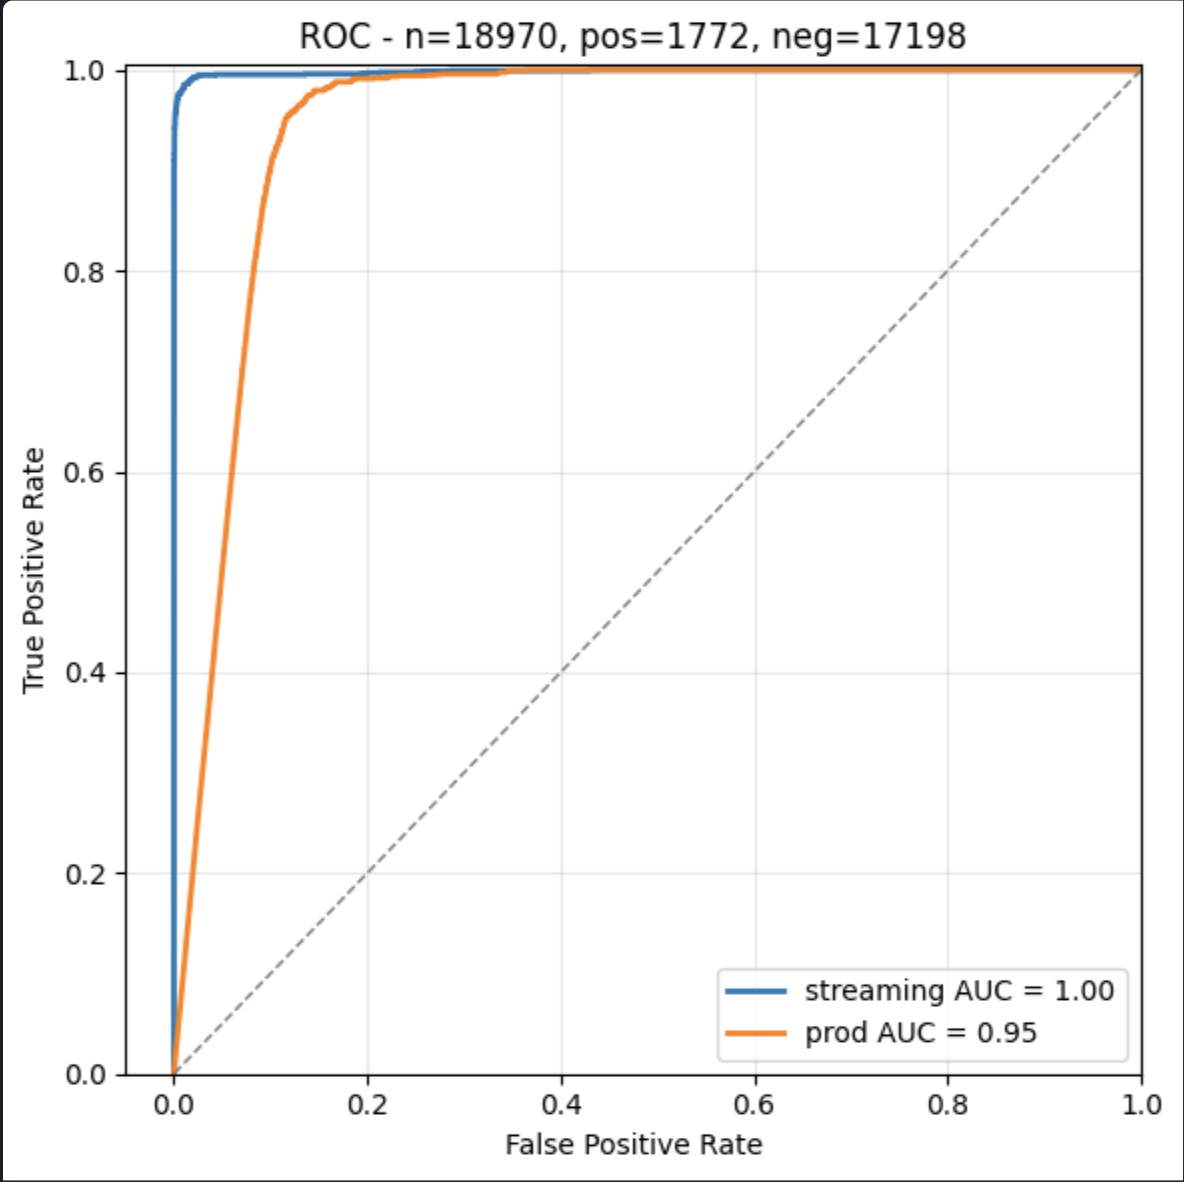
\includegraphics[width=\textwidth]{chapters/figures/censor_old_test.png}
        \caption{Исходный набор (разметка по запросу).}
        \label{fig:sp_censor_old}
    \end{subfigure}

    \vspace{1.5em}

    \begin{subfigure}{0.62\textwidth}
        \centering
        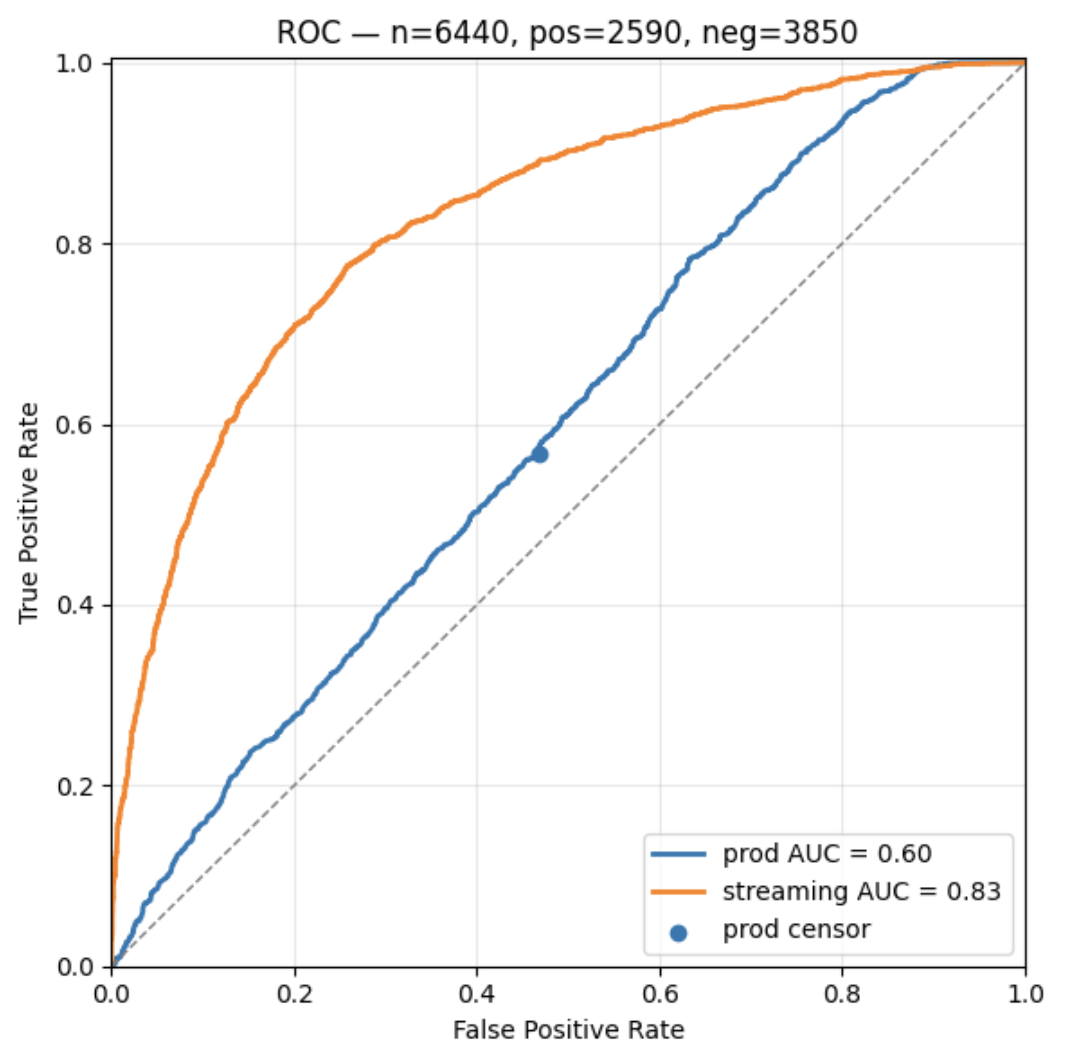
\includegraphics[width=\textwidth]{chapters/figures/censor_new_test.png}
        \caption{Пересмотренный набор (разметка по безопасности ответа).}
        \label{fig:sp_censor_new}
    \end{subfigure}
    \caption{ROC-кривые классификатора запросов (prod) и потокового классификатора ответа (streaming) на исходном и пересмотренном тестовых наборах. Переход к разметке по фактической безопасности ответа выявляет несостоятельность модерации на уровне запроса.}
    \label{fig:sp_censor_roc}
\end{figure}

Рисунок~\ref{fig:sp_censor_roc} сопоставляет ROC-кривые продакшен-классификатора запросов (prod) и потокового классификатора ответа (streaming) на обоих наборах.
На исходном наборе (Рисунок~\ref{fig:sp_censor_old}; $n = 18\,970$, из них $1\,772$ небезопасных и $17\,198$ безопасных обменов) оба классификатора демонстрируют высокое качество --- $\mathrm{AUC} = 0.95$ для классификатора запросов и $\mathrm{AUC} = 1.00$ для потокового, --- что маскирует слабость модерации на уровне запроса.
На пересмотренном наборе (Рисунок~\ref{fig:sp_censor_new}; $n = 6\,440$, из них $2\,590$ небезопасных и $3\,850$ безопасных) качество классификатора запросов падает до $\mathrm{AUC} = 0.60$, приближаясь к случайному угадыванию: его рабочая точка при производственном пороге лежит вблизи диагонали (доля верных обнаружений $\approx 0.57$ при доле ложных срабатываний $\approx 0.47$).
Потоковый классификатор ответа при этом сохраняет существенно более высокую различающую способность ($\mathrm{AUC} = 0.83$).
Полученный разрыв подтверждает, что присвоение метки безопасности обмену, а не изолированному запросу, необходимо для надёжной фильтрации, и обосновывает выбор потоковой классификации ответа в качестве первого этапа конвейера.

Следует подчеркнуть, что, за исключением представленного выше сравнения классификаторов, приведённые в проектной документации значения являются целевыми ориентирами; систематические измерения конвейера в целом составляют предмет дальнейшей работы.

%% =================================================================
\section{Выводы}\label{sec:sp_conclusions}
%% =================================================================

В настоящей главе представлен двухэтапный конвейер обеспечения безопасности мультимодальных больших языковых моделей.
Первый этап --- потоковый классификатор обменов на основе модели GigaChat-10B с архитектурой Mixture of Experts --- выполняет генеративную оценку вредоносности с двухпороговым правилом решения, обеспечивая низкую задержку и независимость от защищаемой модели, и расширяется на визуальную модальность.
Второй этап --- безопасная модель, дообученная методом конституционного ИИ и обучения с подкреплением с гибридной наградой за безопасность, --- формирует неуклончивые ответы, сохраняя баланс между безопасностью и полезностью.
Ключевым элементом конвейера является инструмент безопасного поиска по курируемому индексу, объединяющий поисковый стек, развитый в Главах~\ref{ch:gigaembeddings}--\ref{ch:rag}, с системой обеспечения безопасности и обеспечивающий защищённой модели актуальный и достоверный взгляд на предметную область.
